\documentclass[aspectratio=169]{beamer}

% ---------- Packages ----------
\usepackage[utf8]{inputenc}
\usepackage[T1]{fontenc}
\usepackage{lmodern}
\usepackage{graphicx}
\usepackage{amsmath,amssymb}
\usepackage{siunitx}
\usepackage{booktabs}
\usepackage{xcolor}
\usepackage{hyperref}
\hypersetup{colorlinks=true,linkcolor=blue,urlcolor=blue}

% ---------- Theme ----------
\usetheme{Madrid}
\setbeamertemplate{navigation symbols}{}
\setbeamertemplate{footline}[frame number]

% ---------- Title ----------
\title[Digital Twin (Energy)]{Digital Twin for a Nuclear Primary Loop\\ \small Dynamic Flow + Thermal ROM + EnKF}
\author{Yehua He}
\institute{M2 ROM \& Data-Driven ROM — Université de Strasbourg}
\date{Oct 2025}

\newcommand{\img}[2][]{\includegraphics[width=#1\linewidth]{#2}}

\begin{document}

% ===== 1. TITLE =====
\begin{frame}
  \titlepage
  \vspace{-0.5em}
  \footnotesize
  Devoir Maison 1 — \textit{Jumeau Numérique} \hfill
  Conceptual prototype with simplified physics \& synthetic assimilation
\end{frame}

% ===== 2. PHYSICAL SYSTEM =====
\begin{frame}{Physical System — Primary Loop (Schematic)}
\centering
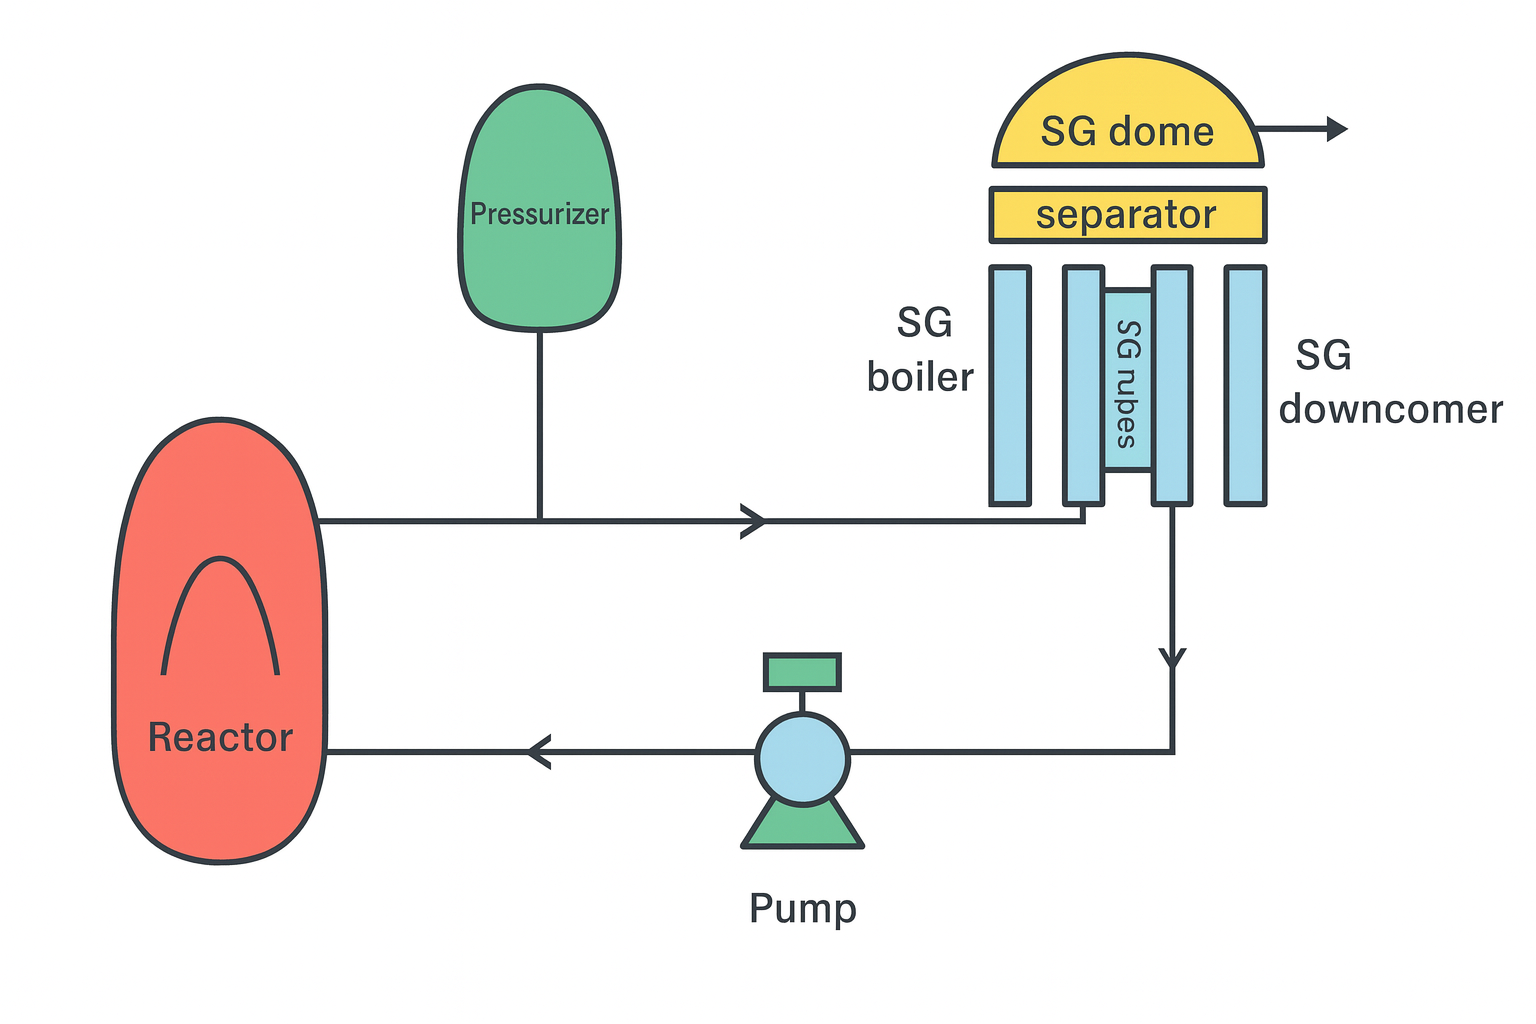
\includegraphics[width=0.8\linewidth]{assets/primary_loop_schematic.png}

\vspace{0.6em}
\footnotesize
Pressurized Water Reactor (PWR) primary loop: Reactor $\rightarrow$ Steam Generator (SG) $\rightarrow$ Pump $\rightarrow$ Reactor.\\
Modeling scope: lumped thermo–hydraulics (0D) with temperatures and mass flow as states.
\end{frame}

% ===== 3. SCOPE & OBJECTIVES =====
\begin{frame}{Scope \& Objectives}
\textbf{Objectives}
\begin{itemize}
  \item Real-time surrogate (ROM) for $T_h,\,T_c,\,\dot m$ with momentum dynamics.
  \item Online data assimilation (EnKF) using temperature measurements.
  \item What-if scenarios: Normal / Pump degraded / Fouled SG.
\end{itemize}

\textbf{Notes (honest)}
\begin{itemize}
  \item Conceptual prototype: 0D single-phase, constant properties; synthetic data.
  \item Aligned with digital twin frameworks for nuclear systems \cite{Liu2024_DigitalTwinNuclear,NRC2021_DigitalTwinChallenges}.
\end{itemize}
\end{frame}

% ===== 4. METHODS — ROM =====
\begin{frame}{Reduced-Order Model (3 ODEs)}
\small
\textbf{State:} $x=[T_h,\,T_c,\,\dot m]^\top$ \hfill explicit Euler.

\medskip
\textbf{Hydraulics (momentum):}
\[
L \frac{d\dot m}{dt}=\Delta P_{\text{pump}}(\dot m)-\Delta P_{\text{loss}}(\dot m),\quad
\Delta P_{\text{pump}}=a_0+a_1\dot m + a_2 \dot m^2,\quad
\Delta P_{\text{loss}}=k_{\text{sys}}\dot m^2
\]

\textbf{Thermal balances:}
\[
\begin{aligned}
M_h c_p \dot T_h &= \dot m c_p (T_c-T_h)+Q_{\text{core}},\\
M_c c_p \dot T_c &= \dot m c_p (T_h-T_c)-UA(T_h-T_{\text{sec}})
\end{aligned}
\]

\medskip
\footnotesize
Projection-based ROM and hyper-reduction references: \cite{Benner2015,Quarteroni2016,Barrault2004,Chaturantabut2010}.

\smallskip
\textbf{ROM type:} physics-based lumped 0D model (not RB/POD); chosen for real-time feasibility and clarity of coupling with EnKF.

\end{frame}

% ===== 5. METHODS — ENKF =====
\begin{frame}{Data Assimilation — Ensemble Kalman Filter}
\small
\textbf{Observations:} $y=[T_h,T_c]^\top$ with Gaussian noise; $\dot m$ unobserved.\\
\textbf{Forecast:} propagate $N_{\text{ens}}$ members via ROM; jitter on $UA,k_{\text{sys}}$ (process noise).\\
\textbf{Analysis:} $K=P_fH^\top(HP_fH^\top+R)^{-1}$; update $T_h,T_c$, and indirectly correct $\dot m$.\\

\medskip
\footnotesize
EnKF theory and practice: \cite{Evensen2009_EnKF}.\\
ROM-based data assimilation and surrogate-enhanced EnKF: \cite{Kovachki2022_MultifidelityEnKF,Maday2015}.
\end{frame}

% ===== 6. ARCHITECTURE =====
\begin{frame}{Architecture \& Pipeline (Conceptual Prototype)}
\centering
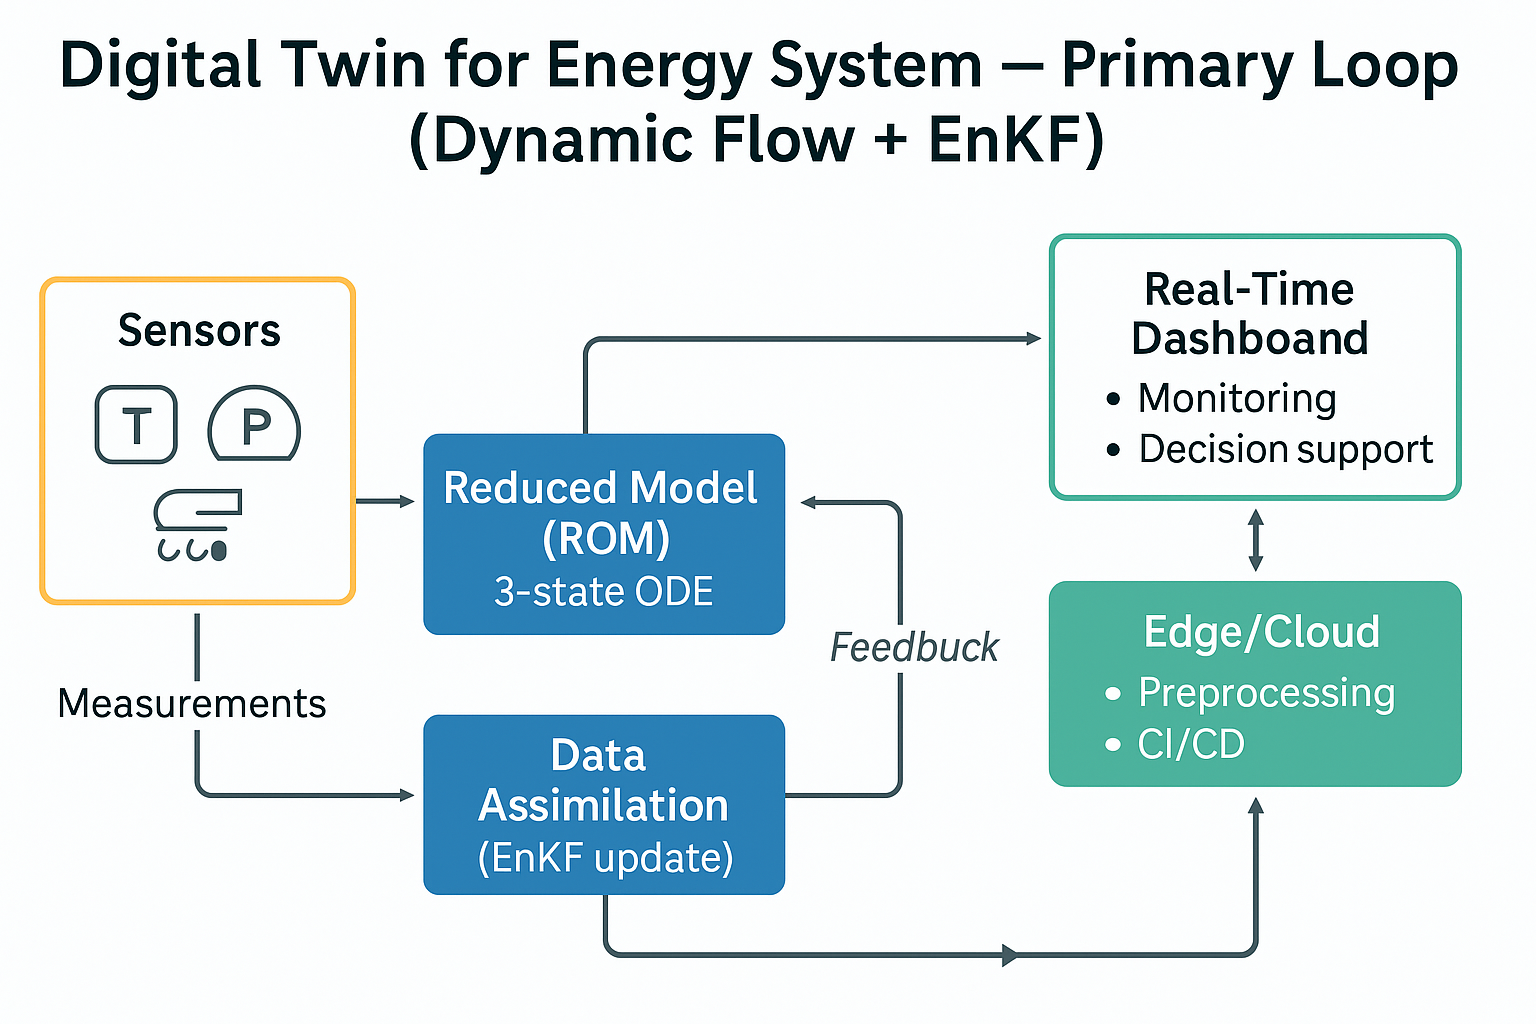
\includegraphics[width=0.8\linewidth]{assets/arch_twin_energy.png}

\vspace{0.6em}
\footnotesize
Physical sensors $\rightarrow$ edge ingestion/preprocessing $\rightarrow$ ROM + EnKF online service $\rightarrow$ cloud archive, dashboard, CI/CD.\\
Conceptual alignment with nuclear DT frameworks \cite{Liu2024_DigitalTwinNuclear,Xiong2025_DeepONetTwin,NRC2021_DigitalTwinChallenges}.
\end{frame}

% ===== 7. RESULTS — HYDRAULICS =====
\begin{frame}{Results — Hydraulics}
\begin{columns}[T,onlytextwidth]
\column{0.5\textwidth}
\img[0.98]{assets/fig_flow_cases_dynamic.png}\\[-0.2em]
\footnotesize Flow $\dot m(t)$ under scenarios.
\column{0.5\textwidth}
\img[0.98]{assets/fig_dpump_cases_dynamic.png}\\[-0.2em]
\footnotesize Pump head $\Delta P_{\text{pump}}(t)$.
\end{columns}
\medskip
\footnotesize
Fouled SG slightly modifies the thermal path, while degraded pump reduces flow stability.
\end{frame}

% ===== 8. RESULTS — THERMAL =====
\begin{frame}{Results — Thermal Evolution}
\centering
\img[0.9]{assets/fig_temperature_dynamic.png}\\[-0.2em]
\footnotesize Hot-leg temperature $T_h(t)$ for Normal / Pump-degraded / Fouled-SG.
\end{frame}

% ===== 9. RESULTS — ENKF =====
\begin{frame}{Results — Assimilation (EnKF)}
\begin{columns}[T,onlytextwidth]
\column{0.5\textwidth}
\img[0.98]{assets/fig_enkf_dynamic_Normal_Th.png}\\[-0.2em]
\footnotesize $T_h$: model vs measurement vs assimilated (95\% CI).
\column{0.5\textwidth}
\img[0.98]{assets/fig_enkf_dynamic_Normal_mdot.png}\\[-0.2em]
\footnotesize Flow $\dot m$: model mean vs assimilated mean.
\end{columns}
\medskip
\footnotesize Assimilation reduces RMSE(model)$\rightarrow$RMSE(assim) by factor $\sim$2--3.
\end{frame}

% ===== 10. V&V & UQ =====
\begin{frame}{Verification \& Uncertainty Quantification}
\begin{columns}[T,onlytextwidth]
\column{0.5\textwidth}
\img[0.98]{assets/fig_verification_dynamic_Th.png}\\[-0.2em]
\footnotesize Step-halving on $T_h$ (rel-$L^2\sim10^{-6}$–$10^{-5}$).
\column{0.5\textwidth}
\img[0.98]{assets/fig_verification_dynamic_mdot.png}\\[-0.2em]
\footnotesize Step-halving on $\dot m$ (consistent convergence).
\end{columns}
\end{frame}

% ===== 11. DATA BUDGET =====
\begin{frame}{Data Budget \& Deployment}
\begin{columns}[T,onlytextwidth]
\column{0.58\textwidth}
\footnotesize
\begin{tabular}{lrrrrr}
\toprule
Sensor & \# & Hz & B/sa. & kB/s & GB/day \\
\midrule
Thermocouple & 40 & 1    & 8  & 0.31 & 0.026 \\
Pressure Tx  & 12 & 10   & 8  & 0.94 & 0.077 \\
Flowmeter    & 4  & 5    & 8  & 0.16 & 0.013 \\
Accel (raw)  & 8  & 2000 & 4  & 62.50 & 5.150 \\
Mic (raw)    & 4  & 8000 & 2  & 62.50 & 5.150 \\
DCS events   & 1  & 1    & 200& 0.20 & 0.016 \\
\midrule
\textit{Subtotal (raw)} & & & & \textit{126.61} & \textit{10.43} \\
\midrule
\textit{Accel (features)} & 8 & 200 & 16 & 25.00 & 2.060 \\
\textit{Mic (features)}   & 4 & 800 & 16 & 50.00 & 4.120 \\
\textit{Subtotal (edge)}  & & & & \textit{75.00} & \textit{6.26} \\
\bottomrule
\end{tabular}


\textcolor{gray}{\footnotesize Edge features (200/800 Hz, 16 B) $\Rightarrow \sim10\times$ reduction; RGPD-safe.}
\column{0.42\textwidth}
\footnotesize
\textbf{Offline}
\begin{itemize}
  \item Parameter calibration, baseline setup.
\end{itemize}
\textbf{Online}
\begin{itemize}
  \item ROM + EnKF $<\,$\SI{10}{ms}/step (CPU).
  \item Logs: performance \& RMSE (JSON/CSV).
\end{itemize}
\textbf{Edge vs Cloud}
\begin{itemize}
  \item Edge: preprocessing, assimilation, alarms.
  \item Cloud: storage, retraining, dashboard, CI/CD.
\end{itemize}
\end{columns}
\end{frame}

% ===== 12. LIMITS & PERSPECTIVES =====
\begin{frame}{Limits \& Perspectives}
\textbf{Limits}
\begin{itemize}
  \item 0D single-phase; no valve/control dynamics; synthetic observations.
\end{itemize}
\textbf{Next}
\begin{itemize}
  \item 1D section model; temperature-dependent properties.
  \item Joint state-parameter DA (augment with $UA,k_{\text{sys}}$).
\end{itemize}
\end{frame}

% ===== 13. REFERENCES (BIBTEX) =====
\begin{frame}{References}
\tiny
\setlength{\itemsep}{0pt}
\setlength{\parskip}{0pt}
\setlength{\parsep}{0pt}
\bibliographystyle{ieeetr}
\bibliography{refs_twin_energy}
\end{frame}

\end{document}
